\chapter{Ubuntu}

\diary{27/12/2017: Lại dính lỗi không thể login. Lần này thì lại phải xóa bạn KDE đi. Kể cũng hơn buồn. Nhưng nhất quyết phải enable được tính năng Windows Spreading (hay đại loại thế). Hóa ra khi ubuntu bị lỗi không có lancher hay toolbar là do bạn unity plugin chưa được enable. Oài. Sao người hiền lành như mình suốt ngày bị mấy lỗi vớ vẩn thế không biết.}

\diary{20/11/2017: Hôm nay đen thật, dính lỗi login loop. Fix mãi mới được. Thôi cũng kệ. Cảm giác bạn KDE này đỡ bị lỗi ibus-unikey hơn bạn GNOME. Hôm nay cũng đổi bạn zsh theme. Chọn mãi chẳng được bạn nào ổn ổn, nhưng không thể chịu được kiểu suggest lỗi nữa rồi. Đôi khi thấy default vẫn là tốt nhất.}

\diary{21/11/2017: Sau một ngày trải nghiệm KDE, cảm giác giao diện mượt hơn GNOME. Khi overview windows với nhiều màn hình tốt và trực quan hơn. Đặc biệt là không bị lỗi ibus nữa. Đổi terminal cũng cảm giác ổn ổn. Không bị lỗi suggest nữa.}

\textbf{Chuyện terminal}

Terminal là một câu chuyện muôn thưở của bất kì ông coder nào thích customize, đẹp, tiện (và bug kinh hoàng). Hiện tại mình đang thấy combo này khá ổn Terminal (Ubuntu) (Color: Black on white, Build-in schemes: Tango) + zsh + oh-my-zsh (fishy-custom theme). Những features hay ho

\begin{itemize}
  \item Làm việc tốt trên cả Terminal (white background) và embedded terminal của Pycharm (black background)
  \item Hiển thị folder dạng ngắn (chỉ ký tự đầu tiên)
  \item Hiển thị brach của git ở bên phải
\end{itemize}


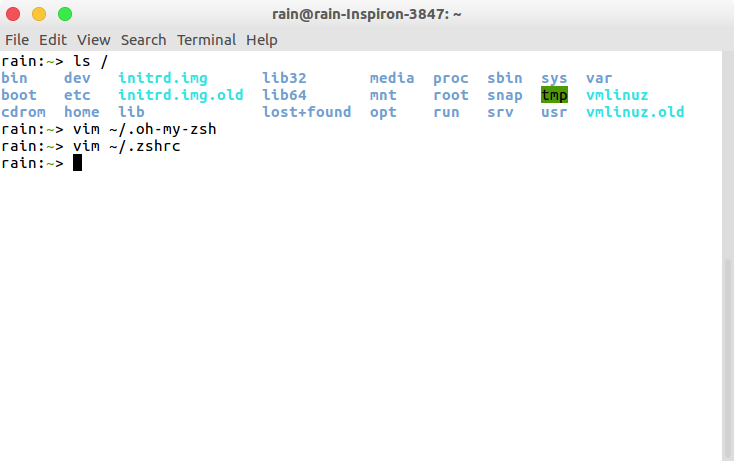
\includegraphics[width=10cm]{images/computer_science/ubuntu/terminal.png}

\textbf{Chuyện bộ gõ}

Làm sao để khởi động lại ibus, thỉnh thoảng lại chết bất đắc kì tử

\begin{lstlisting}
ibus-daemon &
ibus restart
\end{lstlisting}

\textbf{Chuyện lỗi login loop}

Phiên bản: `ubuntu 16.04`



\href{https://askubuntu.com/questions/389903/ibus-doesnt-seem-to-restart}{https://askubuntu.com/questions/389903/ibus-doesnt-seem-to-restart}

\textbf{Hot Corner và Workspace}

Cần cài đặt ngay \textbf{gnome-tweak-tool}

\begin{lstlisting}
sudo apt install gnome-tweak-tool
\end{lstlisting}

Cài đặt hot corner với

\href{https://askubuntu.com/questions/975348/how-to-get-all-hot-corner-in-ubuntu-17-10}{https://askubuntu.com/questions/975348/how-to-get-all-hot-corner-in-ubuntu-17-10}

Cài đặt Workspace

\textbf{Trang game hay}

https://rootgamer.com/how-to/walking-dead-linux-wine

Có lẽ nào trên ubuntu vẫn chơi được game crack như trên Windows. Haha